\documentclass[a4paper,12pt]{article}

\author{Sof\'ia Bel\'en L\'opez Vicens}
\title{Calculation of Density in the SPH Method using Parallel Programming}

\usepackage[utf8]{inputenc}
\usepackage{graphicx}
\usepackage{float}
\usepackage[T1]{fontenc}
\usepackage{textcomp}
\usepackage{amsmath, amssymb}

\begin{document}
\maketitle
\section{Calculation of Density}

\begin{figure}[H]
    \centering
    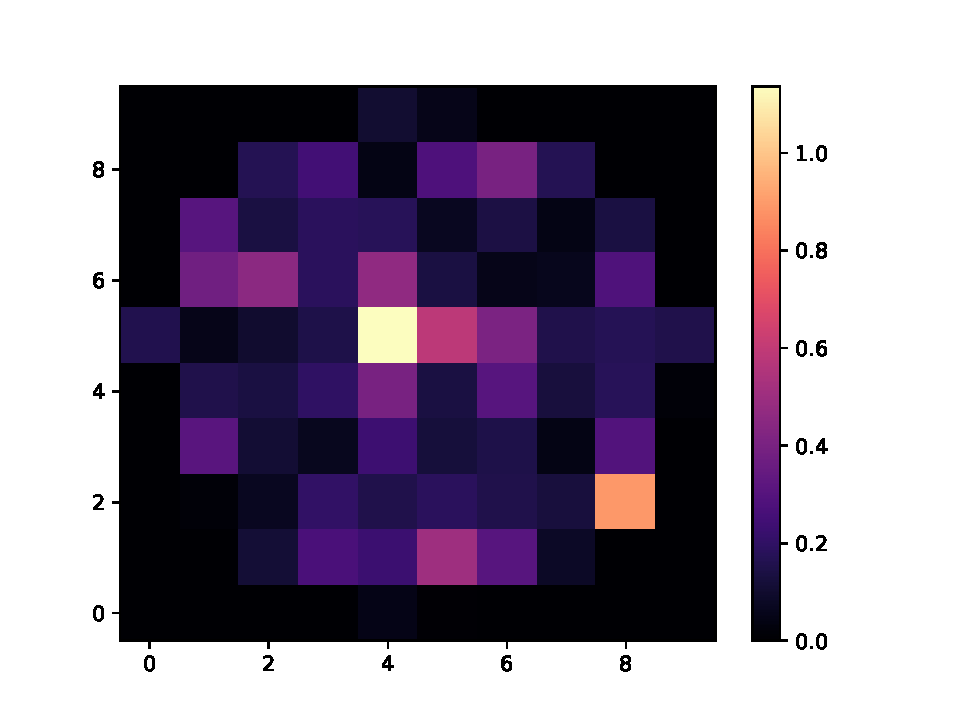
\includegraphics[width=0.8\textwidth]{../img/graph10.pdf}
    \caption{$N_x = N_z = 10$}
\end{figure}

\begin{figure}[H]
    \centering
    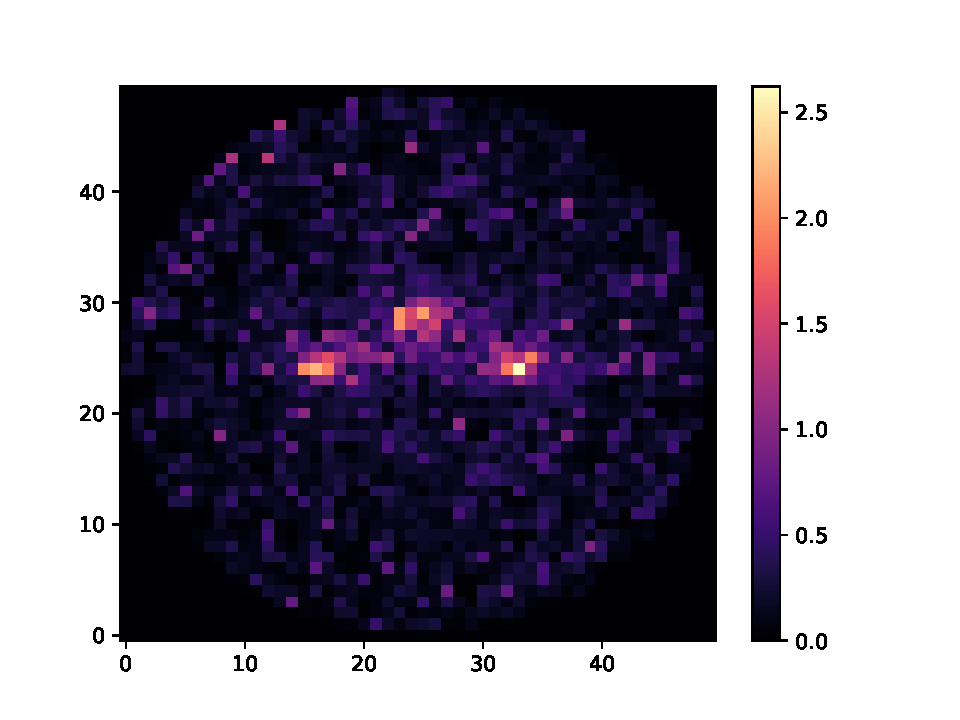
\includegraphics[width=0.8\textwidth]{../img/graph50.pdf}
    \caption{$N_x = N_z = 50$}
\end{figure}

\begin{figure}[H]
    \centering
    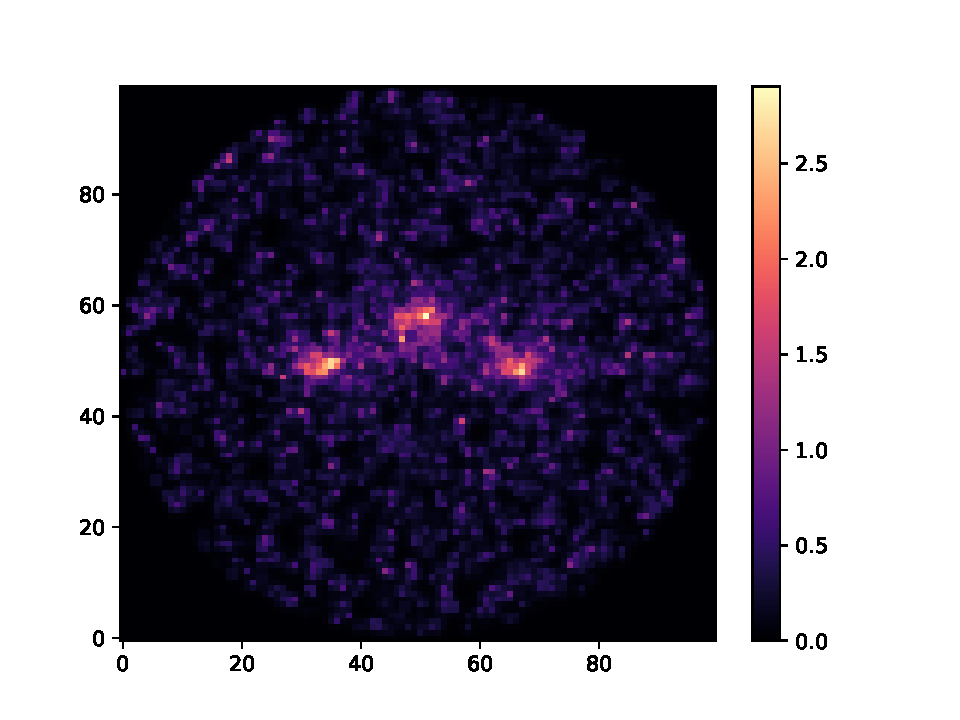
\includegraphics[width=0.8\textwidth]{../img/graph100.pdf}
    \caption{$N_x = N_z = 100$}
\end{figure}
    
\end{document}
